%% This file was auto-generated by IPython.
%% Conversion from the original notebook file:
%% kmeans.ipynb
%%
\documentclass[11pt,english,fleqn]{article}

%% This is the automatic preamble used by IPython.  Note that it does *not*
%% include a documentclass declaration, that is added at runtime to the overall
%% document.

\usepackage{amsmath}
\usepackage{amssymb}
\usepackage{graphicx}
\usepackage{ucs}
\usepackage[utf8x]{inputenc}

% needed for markdown enumerations to work
\usepackage{enumerate}

% Slightly bigger margins than the latex defaults
\usepackage{geometry}
\geometry{verbose,tmargin=3cm,bmargin=3cm,lmargin=2.5cm,rmargin=2.5cm}

% Define a few colors for use in code, links and cell shading
\usepackage{color}
\definecolor{orange}{cmyk}{0,0.4,0.8,0.2}
\definecolor{darkorange}{rgb}{.71,0.21,0.01}
\definecolor{darkgreen}{rgb}{.12,.54,.11}
\definecolor{myteal}{rgb}{.26, .44, .56}
\definecolor{gray}{gray}{0.45}
\definecolor{lightgray}{gray}{.95}
\definecolor{mediumgray}{gray}{.8}
\definecolor{inputbackground}{rgb}{.95, .95, .85}
\definecolor{outputbackground}{rgb}{.95, .95, .95}
\definecolor{traceback}{rgb}{1, .95, .95}

% Framed environments for code cells (inputs, outputs, errors, ...).  The
% various uses of \unskip (or not) at the end were fine-tuned by hand, so don't
% randomly change them unless you're sure of the effect it will have.
\usepackage{framed}

% remove extraneous vertical space in boxes
\setlength\fboxsep{0pt}

% codecell is the whole input+output set of blocks that a Code cell can
% generate.

% TODO: unfortunately, it seems that using a framed codecell environment breaks
% the ability of the frames inside of it to be broken across pages.  This
% causes at least the problem of having lots of empty space at the bottom of
% pages as new frames are moved to the next page, and if a single frame is too
% long to fit on a page, will completely stop latex from compiling the
% document.  So unless we figure out a solution to this, we'll have to instead
% leave the codecell env. as empty.  I'm keeping the original codecell
% definition here (a thin vertical bar) for reference, in case we find a
% solution to the page break issue.

%% \newenvironment{codecell}{%
%%     \def\FrameCommand{\color{mediumgray} \vrule width 1pt \hspace{5pt}}%
%%    \MakeFramed{\vspace{-0.5em}}}
%%  {\unskip\endMakeFramed}

% For now, make this a no-op...
\newenvironment{codecell}{}

 \newenvironment{codeinput}{%
   \def\FrameCommand{\colorbox{inputbackground}}%
   \MakeFramed{\advance\hsize-\width \FrameRestore}}
 {\unskip\endMakeFramed}

\newenvironment{codeoutput}{%
   \def\FrameCommand{\colorbox{outputbackground}}%
   \vspace{-1.4em}
   \MakeFramed{\advance\hsize-\width \FrameRestore}}
 {\unskip\medskip\endMakeFramed}

\newenvironment{traceback}{%
   \def\FrameCommand{\colorbox{traceback}}%
   \MakeFramed{\advance\hsize-\width \FrameRestore}}
 {\endMakeFramed}

% Use and configure listings package for nicely formatted code
\usepackage{listingsutf8}
\lstset{
  language=python,
  inputencoding=utf8x,
  extendedchars=\true,
  aboveskip=\smallskipamount,
  belowskip=\smallskipamount,
  xleftmargin=2mm,
  breaklines=true,
  basicstyle=\small \ttfamily,
  showstringspaces=false,
  keywordstyle=\color{blue}\bfseries,
  commentstyle=\color{myteal},
  stringstyle=\color{darkgreen},
  identifierstyle=\color{darkorange},
  columns=fullflexible,  % tighter character kerning, like verb
}

% The hyperref package gives us a pdf with properly built
% internal navigation ('pdf bookmarks' for the table of contents,
% internal cross-reference links, web links for URLs, etc.)
\usepackage{hyperref}
\hypersetup{
  breaklinks=true,  % so long urls are correctly broken across lines
  colorlinks=true,
  urlcolor=blue,
  linkcolor=darkorange,
  citecolor=darkgreen,
  }

% hardcode size of all verbatim environments to be a bit smaller
\makeatletter 
\g@addto@macro\@verbatim\small\topsep=0.5em\partopsep=0pt
\makeatother 

% Prevent overflowing lines due to urls and other hard-to-break entities.
\sloppy

\setlength{\mathindent}{0pt}
\setlength{\parindent}{0pt}
\setlength{\parskip}{8pt}
\begin{document}

K-Means Kumeleme Metodu

Yapay Ogrenim (Machine Learning) alaninda onemli algoritmalardan biri
k-means metodu. K-means kumelemesi icin kac tane kumenin olmasi
gerektigi bastan tanimlanir (yani k parametresi), algoritma bunu kendisi
bulmaz.

Metotun geri kalani basittir - bir dongu (iteration) icinde her
basamakta:

\begin{enumerate}[1)]
\item
  Her nokta icin, eldeki kume merkezleri teker teker kontrol edilir ve o
  nokta en yakin olan kumeye atanir
\item
  Atamalar tamamlandiktan sonra her kume icinde hangi noktalarin oldugu
  bilindigi icin her kumedeki noktalarin ortalamasi alinarak yeni kume
  merkezi hesaplanir. Eski merkez hesaplari atilir.
\item
  Basa donulur
\end{enumerate}
Dongu tekrar ilk adima dondugunde, bu sefer yeni kume merkezlerini
kullanilarak, ayni adimlar tekrar yapilacaktir.

Fakat bir problem yok mu? Daha birinci dongu baslamadan kume
merkezlerinin nerede oldugunu nereden bilecegiz? Burada bir
tavuk-yumurta problemi var, kume merkezleri olmadan noktalari
atayamayiz, atama olmadan kume merkezlerini hesaplayamayiz.

Bu probleme pratik bir cozum ilk basta kume merkezlerini tahmin
etmektir. Yani merkezleri rasgele bir sekilde hesaplamak. Pratikte bu
yontem cok iyi isliyor. Tabii bu rasgelelik yuzunden K-means'in dogru
sonuca yaklasiksallasi (convergence) garanti degildir, ama gercek dunya
uygulamalarinda cogunlukla kullanisli kumeler bulunur. Bu potansiyel
problemlerden kacinmak icin k-means pek cok kez isletilebilir (her
seferinde yeni rasgele baslangiclarla yani) ve ayni sonuca ulasilip
ulasilmadigi kontrol edilebilir.

Pek en iyi k nasil bulunur? Burada da yapay ogrenim literaturunde pek
cok yaklasim vardir {[}1{]}, veriyi pek cok parcaya bolup, farkli k kume
sayisi icin kumeleme yapmak ve capraz saglama (cross-validation)
kullanmak, vs.

Ornek test verisi altta

\begin{codecell}
\begin{codeinput}
\begin{lstlisting}
from pandas import *
data = read_csv("synthetic.txt",names=['a','b'],sep="   ")
print data.shape
\end{lstlisting}
\end{codeinput}
\begin{codeoutput}
\begin{verbatim}
(3000, 2)
\end{verbatim}
\end{codeoutput}
\end{codecell}
\begin{codecell}
\begin{codeinput}
\begin{lstlisting}
data = np.array(data)
scatter(data[:,0],data[:,1])
\end{lstlisting}
\end{codeinput}
\begin{codeoutput}
\begin{verbatim}
<matplotlib.collections.PathCollection at 0xa371b8c>
\end{verbatim}
\begin{center}
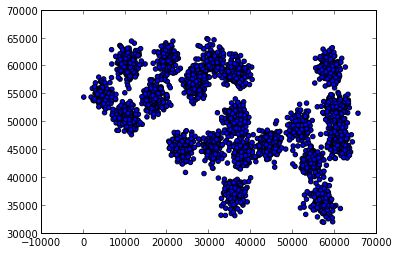
\includegraphics[width=0.7\textwidth]{kmeans_files/kmeans_fig_00.png}
\par
\end{center}
\end{codeoutput}
\end{codecell}
\begin{codecell}
\begin{codeinput}
\begin{lstlisting}
def find_nearest(X,mu):
    nexamples = X.shape[0]
    k = mu.shape[0]
    
    Xmu = dot(X,mu.T)
    xx = sum(X*X,axis=1)
    mm = sum(mu*mu, axis=1)
    
    cl = empty(nexamples,dtype=int)
    dists = inf * ones(nexamples)
    for i in range(k):
        new_dist = - 2*Xmu[:,i] + mm[i]
        change = new_dist < dists
        if sum(change)>0:
            cl[change] = [i for j in range(sum(change))]
            dists[change] = new_dist[change]
    return cl

def kmeans(X, k=5, niter=100):
    nexamples,nfeatures = X.shape
    
    # intialize with a random clustering
    random.seed(1) # seed random number generator for reproducibility
    cl = random_integers(0,k,nexamples)
    cl_old = cl
    
    # allocate means
    mu = np.empty((k,nfeatures))
    
    it = 0
    while True:
        # compute means
        for i in range(k):
            mu[i,:] = np.mean(X[cl==i,:],axis=0)
        
        # assign examples to clusters
        cl = find_nearest(X, mu)
        
        # compute difference in assignments
        nchanges = sum(cl != cl_old)
        print 'it: %d, num. changes: %d' % (it, nchanges)
        if nchanges == 0 or it == niter:
            break
        
        cl_old = cl
        it += 1
    return cl, mu
\end{lstlisting}
\end{codeinput}
\end{codecell}
\begin{codecell}
\begin{codeinput}
\begin{lstlisting}
c = kmeans(data)
\end{lstlisting}
\end{codeinput}
\begin{codeoutput}
\begin{verbatim}
it: 0, num. changes: 2490
it: 1, num. changes: 561
it: 2, num. changes: 277
it: 3, num. changes: 142
it: 4, num. changes: 50
it: 5, num. changes: 32
it: 6, num. changes: 35
it: 7, num. changes: 33
it: 8, num. changes: 24
it: 9, num. changes: 13
it: 10, num. changes: 6
it: 11, num. changes: 2
\end{verbatim}
\begin{verbatim}
it: 12, num. changes: 0
\end{verbatim}
\end{codeoutput}
\end{codecell}
\begin{codecell}
\begin{codeinput}
\begin{lstlisting}
c
\end{lstlisting}
\end{codeinput}
\begin{codeoutput}
\begin{verbatim}
(array([4, 4, 4, ..., 1, 1, 1]),
 array([[ 31006.2193159 ,  58653.75251509],
       [ 12247.38927098,  56210.74828061],
       [ 38859.46193772,  44285.88408304],
       [ 27194.63636364,  45613.61279461],
       [ 57107.29855716,  47792.74694784]]))
\end{verbatim}
\end{codeoutput}
\end{codecell}
Ustteki sonucun icinde iki ana vektor var, bu vektorlerden birincisi
icinde 4,1, gibi sayilar goruluyor, bu sayilar her noktaya tekabul eden
kume atamalari. Ikinci vektor icinde iki boyutlu k tane vektor var, bu
vektorler de her kumenin merkez noktasi. Merkez noktalarini ham veri
uzerinde grafiklersek (kirmizi noktalar)

\begin{codecell}
\begin{codeinput}
\begin{lstlisting}
scatter(data[:,0],data[:,1])
plt.hold(True)
for x in c[1]: plot(x[0],x[1],'rd')
    
\end{lstlisting}
\end{codeinput}
\begin{codeoutput}
\begin{center}
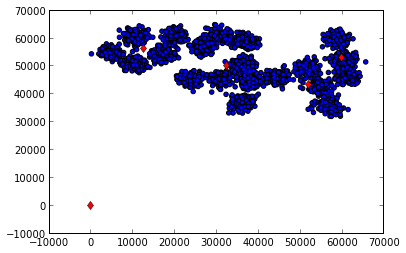
\includegraphics[width=0.7\textwidth]{kmeans_files/kmeans_fig_01.png}
\par
\end{center}
\end{codeoutput}
\end{codecell}
Goruldugu gibi 5 tane kume icin ustteki merkezler bulundu. Fena degil.
Eger 10 dersek

\begin{codecell}
\begin{codeinput}
\begin{lstlisting}
c = kmeans(data,k=10)
scatter(data[:,0],data[:,1])
plt.hold(True)
for x in c[1]: plot(x[0],x[1],'rd')
\end{lstlisting}
\end{codeinput}
\begin{codeoutput}
\begin{verbatim}
it: 0, num. changes: 2683
it: 1, num. changes: 706
it: 2, num. changes: 648
it: 3, num. changes: 262
it: 4, num. changes: 152
it: 5, num. changes: 133
it: 6, num. changes: 132
it: 7, num. changes: 118
it: 8, num. changes: 90
\end{verbatim}
\begin{verbatim}
it: 9, num. changes: 71
it: 10, num. changes: 40
it: 11, num. changes: 20
it: 12, num. changes: 12
it: 13, num. changes: 15
it: 14, num. changes: 11
it: 15, num. changes: 10
it: 16, num. changes: 9
it: 17, num. changes: 7
\end{verbatim}
\begin{verbatim}
it: 18, num. changes: 6
it: 19, num. changes: 4
it: 20, num. changes: 6
it: 21, num. changes: 4
it: 22, num. changes: 0
\end{verbatim}
\begin{center}
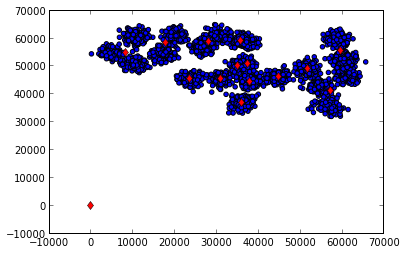
\includegraphics[width=0.7\textwidth]{kmeans_files/kmeans_fig_02.png}
\par
\end{center}
\end{codeoutput}
\end{codecell}
{[}1{]}
http://en.wikipedia.org/wiki/Determining\_the\_number\_of\_clusters\_in\_a\_data\_set

{[}2{]}
nbviewer.ipython.org/url/cbcb.umd.edu/\ensuremath{\sim}hcorrada/PML/src/kmeans.ipynb

\end{document}
